\begin{frame}
\frametitle{Конкуррентное исполнение}
\begin{figure}
  \centering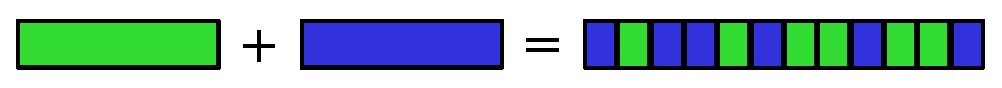
\includegraphics[width=.8\linewidth]{concurrency}
  \caption{Concurrent Execution}
\end{figure}

Конкурентное исполнение - исполняющиеся участки кода нкаладываются друг на
друга произвольным образом

\begin{itemize}
  \item вы не должны делать никаких предположений о порядке наложения;
  \item произвольный порядок ведет к проивольному досутупу к общим ресурсам;
\end{itemize}
\end{frame}

\begin{frame}
\frametitle{Конкуррентное исполнение}
\framesubtitle{Источники конкуррентности}

\begin{itemize}
  \item<1-> много агентов исполняющих код:
        \begin{itemize}
          \item Hyper Threading, SMP, NUMA (shared memory);
          \item cluster nodes (shared storage);
        \end{itemize}
  \item<2-> прерывания - прерывают один код и запускают исполнение другого;
  \item<3-> сигналы - userspace аналог прерываний.
\end{itemize}
\end{frame}

\begin{frame}[fragile]
\frametitle{Конкурретное исполнение}
\framesubtitle{Состояние гонки}

\begin{columns}[T]
  \begin{column}{.45\linewidth}
    \begin{lstlisting}
int cnt;

void foo(void)
{
  ++cnt;
}
    \end{lstlisting}
  \end{column}
  \begin{column}{.45\linewidth}
    \begin{lstlisting}
extern int cnt;

void bar(void)
{
  ++cnt;
}
    \end{lstlisting}
  \end{column}
\end{columns}
\end{frame}

\begin{frame}[fragile]
\frametitle{Конкурретное исполнение}
\framesubtitle{Состояние гонки}

\begin{columns}[T]
  \begin{column}{.45\linewidth}
    \begin{lstlisting}
  .global cnt
cnt:
  .int 0

foo:
  mov cnt, %rax
  inc %rax
  mov %rax, cnt
  ret
    \end{lstlisting}
  \end{column}
  \begin{column}{.45\linewidth}
    \begin{lstlisting}
  .extern cnt

bar:
  mov cnt, %rax
  inc %rax
  mov %rax, cnt
  ret
    \end{lstlisting}
  \end{column}
\end{columns}
\end{frame}

\begin{frame}
\frametitle{Взаимное исключение}

Взаимное исключение (Mutual Exclusion) - позволяет оградить критическую секцию,
чтобы предотвратить конкуренции

\begin{itemize}
  \item lock и unlock - ограничивают критическую секции в начале и конце
        соответсвенно;
  \item только один поток исполнения может находиться в критической секции
        \begin{itemize}
          \item lock не вернет управление, до тех пор, пока поток в критической
                секции не сделает unlock;
        \end{itemize}
  \item если в критической секции не находитс поток, то из нескольких
        конкурирующих lock-ов, как миниум один будет успешным;
\end{itemize}
\end{frame}

\begin{frame}
\frametitle{Взаимное исключение}

Мы можем считать, что
\begin{itemize}
  \item поток выйдет из критической секции за конечное время
        \begin{itemize}
          \item поток не зависнет и не упадет внутри критической секции;
        \end{itemize}
\end{itemize}

\onslide<2->{Мы не можем делать предположений о
\begin{itemize}
  \item скорости работы потока
        \begin{itemize}
          \item время нахождения в критической секции конечно, но ограничение
                сверху нам не известно;
        \end{itemize}
  \item взаимной скорости работы потоков
        \begin{itemize}
          \item мы не можем считать, что один поток быстрее/медленне другого или
                что их скорости равны
        \end{itemize}
\end{itemize}}
\end{frame}

\begin{frame}[fragile]
\frametitle{Реализация взимного исключения}
\framesubtitle{Глобальный флаг}

\begin{columns}[T]
  \begin{column}{.45\linewidth}
    \begin{lstlisting}
extern int claim1;
int claim0;

void lock0()
{
  claim0 = true;
  while (claim1);
}

void unlock0(void)
{
  claim0 = false;
}
    \end{lstlisting}
  \end{column}
  \begin{column}{.45\linewidth}
    \begin{lstlisting}
extern int claim0;
int claim1;

void lock1(void)
{
  claim1 = true;
  while (claim0);
}

void unlock1(void)
{
  claim1 = false;
}
    \end{lstlisting}
  \end{column}
\end{columns}
\end{frame}

\begin{frame}
\frametitle{Реализация взимного исключения}
\framesubtitle{Глобальный флаг}

Следующее расписание приводит к deadlock-у:
\begin{enumerate}
  \item Thread 0, line 6;
  \item Thread 1, line 6;
  \item Thread 0, line 7 (Thread 0 завис на этой строке);
  \item Thread 1, line 7 (Thread 1 завис на этой строке);
\end{enumerate}
\end{frame}

\begin{frame}[fragile]
\frametitle{Реализация взимного исключения}
\framesubtitle{Глобальный порядок}

\begin{columns}[T]
  \begin{column}{.45\linewidth}
    \begin{lstlisting}
int turn;

void lock0(void)
{
  while (turn != 0);
}

void unlock0(void)
{
  turn = 1;
}
    \end{lstlisting}
  \end{column}
  \begin{column}{.45\linewidth}
    \begin{lstlisting}
extern int turn;

void lock1(void)
{
  while (turn != 1);
}

void unlock0(void)
{
  turn = 0;
}
    \end{lstlisting}
  \end{column}
\end{columns}
\end{frame}

\begin{frame}
\frametitle{Реализация взимного исключения}
\framesubtitle{Глобальный порядок}

Расписание приводяещее к проблемам:
\begin{enumerate}
  \item Thread 1, line 5 (Thread 1 завис на этой строке);
  \item Thread 0 - умер (решил не заходить в критическую секцию);
\end{enumerate}
\onslide<2->{Да, оно довольно короткое...}
\end{frame}

\begin{frame}[fragile]
\frametitle{Реализация взимного исключения}
\framesubtitle{Соберем все в кучу}

\begin{columns}[T]
  \begin{column}{.45\linewidth}
    \begin{lstlisting}
extern int claim1;
int claim0;
int turn;

void lock0(void)
{
  claim0 = true;
  turn = 1;

  while (claim1 && turn == 1);
}

void unlock0(void)
{
  claim0 = false;
}
    \end{lstlisting}
  \end{column}
  \begin{column}{.45\linewidth}
    \begin{lstlisting}
extern int claim0;
extern int turn;
int claim1;

void lock1(void)
{
  claim1 = true;
  turn = 0;

  while (claim0 && turn == 0);
}

void unlock1(void)
{
  claim1 = false;
}
    \end{lstlisting}
  \end{column}
\end{columns}
\end{frame}

\begin{frame}
\frametitle{Реализация взаимного исключения}
\framesubtitle{Алгоритм Петтерсона}

\emph{Доказательство взаимного исключения:}
\begin{itemize}
  \item пусть сразу два потока находятся в критической секции:
        \begin{itemize}
          \item turn принимает одно из двух значений: 0 или 1; для
                определенности пусть это будет 0, т. е. последним в turn
                записывал поток 1;
          \item claim0 и claim1 оба равны true;
        \end{itemize}
  \item к моменту проверки условия цикла потоком 1 имеем:
        \begin{itemize}
          \item turn равен 0;
          \item claim0 равнен true;
          \item но в этом случае поток 1 должен зависнуть в цикле до изменения
                turn или claim0 - противорчие;
        \end{itemize}
\end{itemize}
\end{frame}

\begin{frame}
\frametitle{Реализация взаимного исключения}
\framesubtitle{Алгоритм Петтерсона}

\emph{Доказательство наличия прогресса:} пусть поток 0 пытается войти в
свободную критическую секцию:
\begin{itemize}
  \item<1-> поток 0 в 10 строке видит claim1 == true:
        \begin{itemize}
          \item поток 0 видит turn == 0, поток 0 входит в критическую секцию;
          \item поток 0 видит turn == 1, возможны два случая:
                \begin{itemize}
                  \item поток 1 выполнил строку 8, поток 0 перезаписал turn -
                        поток 1 входит в критическую секцию;
                  \item поток 1 собирается выполнить строку 8 - поток 0 войдет в
                        критическую секцию, после того как поток 1 выполнит
                        строку 8;
                \end{itemize}
        \end{itemize}
  \item<2> поток 0 видит claim1 == false - поток 0 входит в критическую секцию;
\end{itemize}
\end{frame}

\begin{frame}[fragile]
\frametitle{Реализация взаимного исключения}
\framesubtitle{Алгоритм Петтерсона для N потоков}

\begin{lstlisting}
int flag[N];
int turn[N - 1];

void lock(int i)
{
  for (int count = 0; count < N - 1; ++count) {
    flag[i] = count + 1;
    turn[count] = i;

    int found = true;
    while (turn[count] == i && found) {
      found = false;
      for (int k = 0; !found && k != N; ++k) {
        if (k == i) continue;
        found = flag[k] > count;
      }
    }
  }
}

void unlock(int i)
{
  flag[i] = 0;
}
\end{lstlisting}
\end{frame}

\begin{frame}
\frametitle{Реализация взаимного исключения}
\framesubtitle{Честность Алгоритма Петтерсона}

\only<1>{Рассмотрим пример на 3 потоках. Начальное состояние:
\begin{itemize}
  \item flag[3] = \{0, 0, 0\};
  \item turn[2] = \{0, 0\};
\end{itemize}}
\only<1>{Поток 0 пытается войти в критическую секцию (count = 0):
\begin{itemize}
  \item flag[3] = \{1, 0, 0\};
  \item turn[2] = \{0, 0\};
\end{itemize}}
\only<2>{Поток 1 пытается войти в критическую секцию (count = 0):
\begin{itemize}
  \item flag[3] = \{1, 1, 0\};
  \item turn[2] = \{1, 0\};
\end{itemize}}
\only<3>{Поток 2 пытается войти в критическую секцию (count = 0):
\begin{itemize}
  \item flag[3] = \{1, 1, 1\};
  \item turn[2] = \{2, 0\};
\end{itemize}}
\only<4>{Поток 1 пытается войти в критическую секцию (count = 1):
\begin{itemize}
  \item flag[3] = \{1, 2, 1\};
  \item turn[2] = \{2, 1\};
\end{itemize}}
\only<5>{Поток 1 вошел в критическую секцию... И вышел из критической секции:
\begin{itemize}
  \item flag[3] = \{1, 0, 1\};
  \item turn[2] = \{2, 1\};
\end{itemize}}
\only<6>{Поток 1 пытается войти в критическую секцию (count = 0):
\begin{itemize}
  \item flag[3] = \{1, 1, 1\};
  \item turn[2] = \{1, 1\};
\end{itemize}}
\only<7>{Поток 2 пытается войти в критическую секцию (count = 1):
\begin{itemize}
  \item flag[3] = \{1, 1, 2\};
  \item turn[2] = \{1, 2\};
\end{itemize}}
\only<8>{Поток 2 вошел в критическую секцию... И вышел из критической секции:
\begin{itemize}
  \item flag[3] = \{1, 1, 0\};
  \item turn[2] = \{1, 2\};
\end{itemize}}
\only<9>{Поток 2 пытается войти в критическую секцию (count = 0):
\begin{itemize}
  \item flag[3] = \{1, 1, 1\};
  \item turn[2] = \{2, 2\};
\end{itemize}}
\only<10>{Поток 1 пытается войти в критическую секцию (count = 1):
\begin{itemize}
  \item flag[3] = \{1, 2, 1\};
  \item turn[2] = \{2, 1\};
\end{itemize}
Мы уже были в этом состоянии! А поток 0 так и не получил управление!}
\end{frame}

\begin{frame}
\frametitle{Реализация взаимного исключения}
\framesubtitle{Алгоритм Пекарни (Л. Лэмпорт)}

\onslide<1->{Каждый поток при попытке входа выбирает себе число:
\begin{itemize}
  \item число определяет место в очереди;
  \item новое число выбирается так, чтобы оно было больше всех чисел в очереди;
\end{itemize}}

\onslide<2->{Как выбирать это число?
\begin{itemize}
  \item посмотреть на числа всех потоков и прибавить 1 к наибольшему;
  \item что если два потока выбирают число одновременно?
\end{itemize}}

\onslide<3->{Как использовать выбранное число?
\begin{itemize}
  \item если число наименьшее среди всех потоков выбравших число, то входим в
        критическую секцию;
\end{itemize}}
\end{frame}

\begin{frame}[fragile]
\frametitle{Реализация взаимного исключения}
\framesubtitle{Алгоритм Пекарни (Л. Лэмпорт)}

\begin{columns}[T]
  \begin{column}{.45\linewidth}
    \begin{lstlisting}
int choosing[N];
int number[N];

int max(void)
{
  int rc = 0;

  for (int i = 0; i != N; ++i) {
    const int n = number[i];

    if (n > rc)
      rc = n;
  }

  return rc;
}

int less(int id0, int n0,
         int id1, int n1)
{
  if (n0 < n1)
    return true;
  if (n0 == n1 && id0 < id1)
    return true;
  return false;
}
    \end{lstlisting}
  \end{column}
  \begin{column}{.45\linewidth}
    \begin{lstlisting}
void lock(int i)
{
  choosing[i] = true;
  number[i] = max() + 1;
  choosing[i] = false;

  for (int j = 0; j != N; ++j) {
    while (choosing[j]);
    while (less(j, number[j], i, number[i]));
  }
}

void unlock(int i)
{
  number[i] = 0;
}
    \end{lstlisting}
  \end{column}
\end{columns}
\end{frame}
